\documentclass[a4paper,fleqn]{article} %Options in documentclass should be set to a4paper and fleqn.
\usepackage{modsim}
\usepackage{times}
\usepackage{psfrag}
 \usepackage{pstricks}
 %\usepackage{auto-pst-pdf}
\usepackage{pstool}
\usepackage{natbib} %The three packages modsim, times and natbib are required.
\usepackage{amsmath, amssymb, amsthm} %Also recommend the standard AMS LaTeX maths packages.
\usepackage{changes}

\newcommand\solidrule[1][0.25cm]{\rule[0.5ex]{#1}{1pt}}
\newcommand\dashedrule{\mbox{%
		\solidrule[2mm]\hspace{2mm}\solidrule[2mm]}}
 \begin{document}

\begin{figure}
	\centering
	\begin{tabular}{ccc}
		\resizebox{5cm}{!}{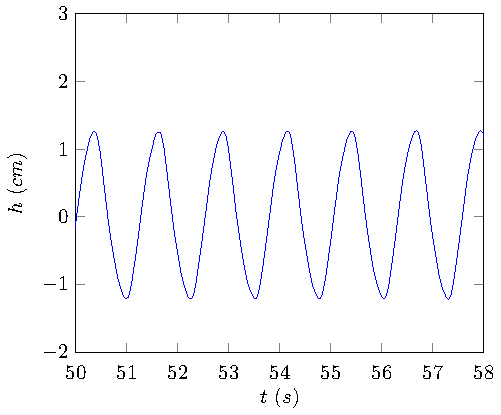
\includegraphics{WG1.pdf}} & & \resizebox{5cm}{!}{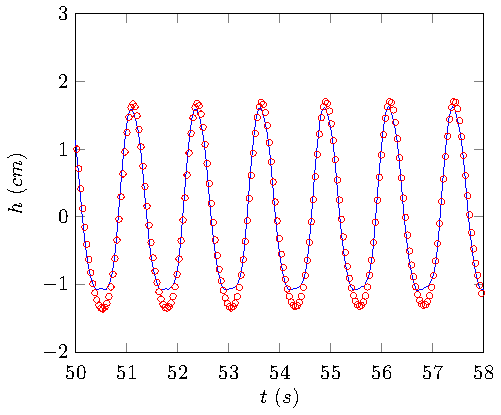
\includegraphics{WG2Serre.pdf}}  \\
		\hspace{5 mm} WG1 & & \hspace{5 mm}WG2 \\
		\resizebox{5cm}{!}{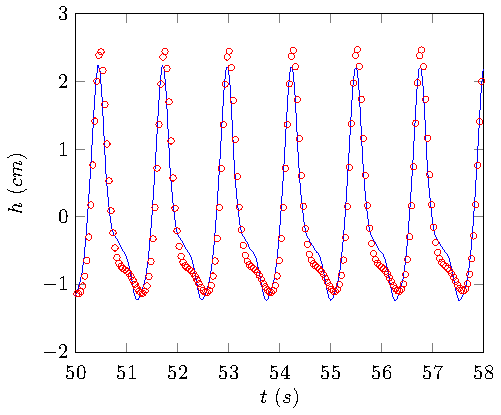
\includegraphics{WG3Serre.pdf}} && 
		\resizebox{5cm}{!}{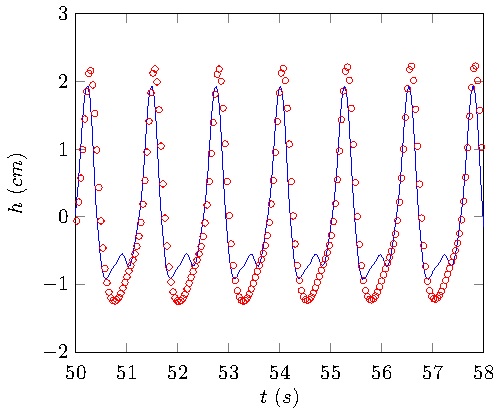
\includegraphics{WG4Serre.pdf}}  \\
		\hspace{5 mm} WG3 & & \hspace{5 mm} WG4 \\
		
		
	\end{tabular}
	\caption{Wave height readings from various wave gauges from the experiment ({\color{blue} \solidrule}) compared to a simulation of the experiment using the Serre equations ({\color{red} $\circ$}).}
	\label{fig:WGSerre}
\end{figure}

\begin{figure}
	\centering
	\begin{tabular}{ccc}
		\resizebox{5cm}{!}{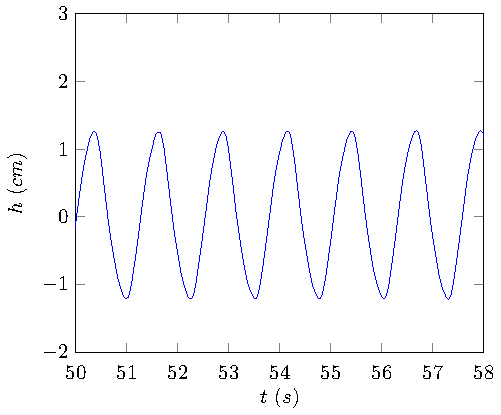
\includegraphics{WG1.pdf}} & & \resizebox{5cm}{!}{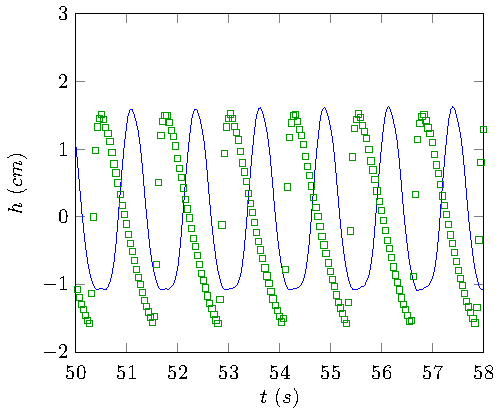
\includegraphics{WG2SWW.pdf}}  \\
		\hspace{5 mm} WG1 & & \hspace{5 mm}WG2 \\
		\resizebox{5cm}{!}{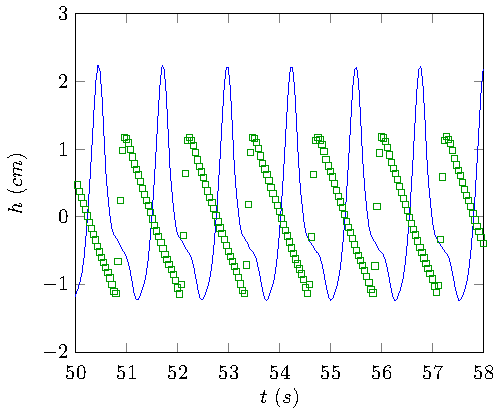
\includegraphics{WG3SWW.pdf}} && 
		\resizebox{5cm}{!}{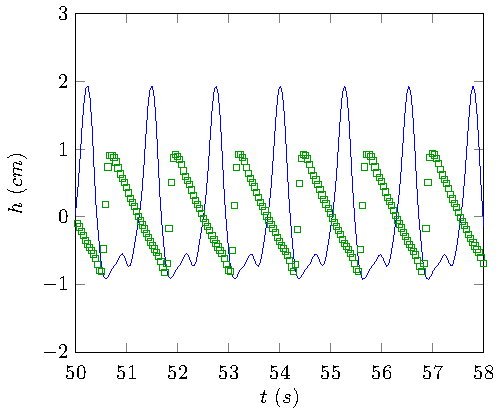
\includegraphics{WG4SWW.pdf}}  \\
		\hspace{5 mm} WG3 & & \hspace{5 mm} WG4 \\
		
		
	\end{tabular}
	\caption{Wave height readings from various wave gauges from the experiment ({\color{blue} \solidrule}) compared to a simulation of the experiment using the shallow water wave equations ({\color{green!60!black} $\square$}).}
	\label{fig:WGSWW}
\end{figure}
	

\end{document}
